\documentclass[a4paper,12pt]{report}
\usepackage[T2A]{fontenc}
\usepackage[utf8]{inputenc}
\usepackage[english,russian]{babel}
\usepackage{graphicx}
\usepackage{wrapfig}
\usepackage{mathtext} 				% русские буквы в фомулах
\usepackage{amsmath,amsfonts,amssymb,amsthm,mathtools} % AMS
\usepackage{icomma} % "Умная" запятая: $0,2$ --- число, $0, 2$ --- перечисление
\usepackage{capt-of}
\usepackage{appendix}
\usepackage{multirow}
\usepackage{hyperref}
\usepackage{floatrow}
\usepackage[left=2cm,right=2cm,
    top=2cm,bottom=2cm,bindingoffset=0cm]{geometry}
\usepackage{multicol} % Несколько колонок
\usepackage{gensymb}
\title{Отчёт по лабораторной работе № 4.7.2 

Эффект Поккельса.}
\author{Плюскова Н.А. Б04-004 }
\date{\today}
\begin{document}
\maketitle
\section*{1. Аннотация}

В данной работе будет исследована интерференция рассеянного света, прошедшего кристалл, а также пронаблюдаем изменение характера поляризации света при наложении на кристалл электрического поля.

\section*{2. Теоретические сведения}

Эффект Поккельса -- изменение показателя преломления света в кристалле под действием электрического поля.\\
Рассмотрим кристалл ниобата лития $\text{LiNbO}_3$ с центральноосевой симметрией вдоль оси $Z$. Для световой волны с $\mathbf{E}$ перпендикулярно $Z$ показатель преломления будет $n_o$, а для волны с $\mathbf{E}$ вдоль $Z$ -- $n_e$. В случае, когда луч света идёт под углом $\theta$ к оси, есть два значение показателя преломления $n_1$ и $n_2$: $n_1 = n_o$ для волны с $\mathbf{E}$ перпендикулярным плоскости $(\mathbf{k},\mathbf{Z})$ (обыкновенная волна) и $n_2$ для волны с $\mathbf{E}$ в этой плоскости (необыкновенная волна). В последнем случае:

\begin{equation}
\dfrac{1}{n_2^2}=\dfrac{\cos^2 \theta}{n_0^2}+\dfrac{\sin^2 \theta}{n_e^2}.
\end{equation}

\begin{figure}[H]
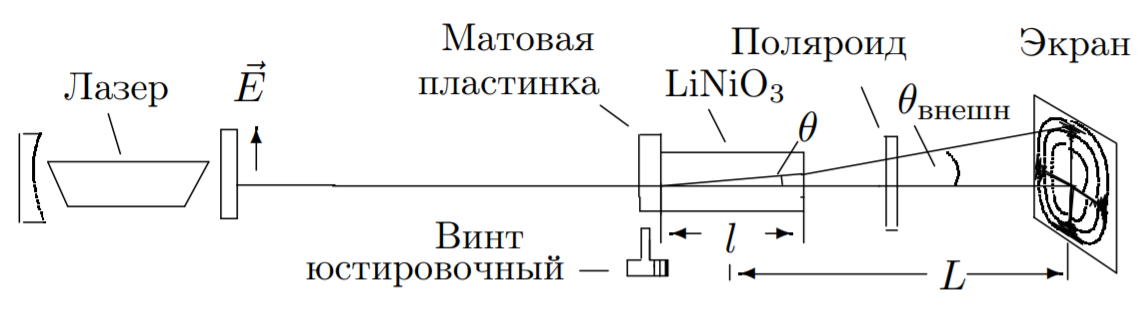
\includegraphics[width = 0.8\textwidth]{1.png}
\centering
\caption{Схема для наблюдения интерференционной картины }
\end{figure}

Если перед кристаллом, помещённым между поляроидами, расположить линзу или матовую пластинку, то на экране за поляроидом мы увидим тёмные концентрические окружности -- результат интерференции обыкновенной и необыкновенной волн. При повороте выходного поляроида на $90^\circ$ картина меняется с позитива на негатив (на месте светлых пятен тёмные и наоборот). В случаи, когда разрешённое направление анализатора перпендикулярно поляризации лазерного излучения, радиус тёмного кольца с номером $m$ равен
\begin{equation}
r_m^2 = \dfrac{\lambda}{l} \dfrac{(n_oL)^2}{n_0 - n_e}m,
\end{equation}
где $L$ -- расстояние от центра кристалла до экрана, $l$ -- длина кристалла.\\
Теперь поместим кристалл в постоянное электрическое поле $E_{\text{эл}}$, направленное вдоль оси $X$, перпендикулярной $Z$. Показатель преломления для луча, распространяющего вдоль $Z$, всегда $n_o$. В плоскости $(X,Y)$ возникают два главных направления под углами $45^\circ$ к $X$ и $Y$ с показателями преломления $n_0 - \Delta n$ и $n_o + \Delta n$ (быстрая и медленная ось), причём $\Delta n = A E_{\text{эл}}$. Для поляризованного вертикально света и анализатора, пропускающего горизонтальную поляризацию, на выходе интенсивность на выходе будет иметь вид
\begin{equation}
I_{\text{вых}} = I_0 \sin^2 \left(\dfrac{\pi}{2} \dfrac{U}{U_{\lambda/2}} \right),
\end{equation}
где $U_{\lambda/2} = \frac{\lambda}{4A}\frac{d}{l}$ -- \textit{полуволновое напряжение}, $d$ -- поперечный размер кристалла.  При напряжении $U = E_{\text{эл}}d$ равном полуволновому сдвиг фаз между двумя волнами равен $\pi$, а интенсивность света на выходе максимальна. 

\begin{figure}[H]
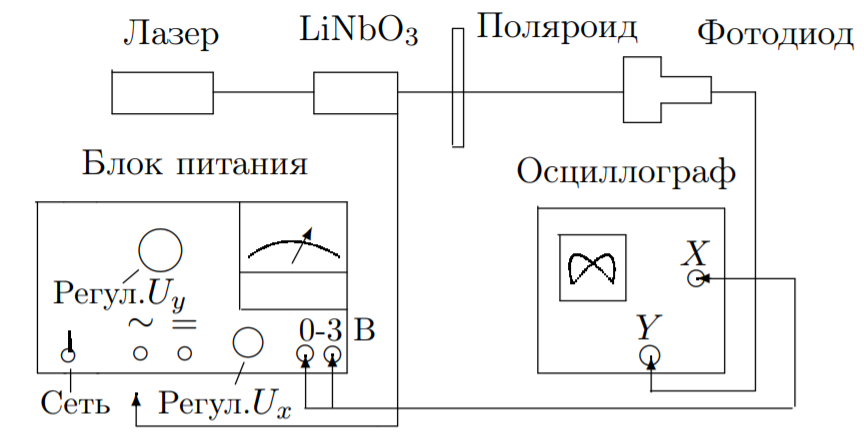
\includegraphics[width = 0.8\textwidth]{2.png}
\centering
\caption{Схема установки}
\end{figure}

На Рис. 2 представлена схема всей установки (оптическая часть изображена на Рис. 1). Свет лазера, проходя через сквозь пластину, рассеивается и падает на двояко преломляющий кристалл. На экране за поляроидом видна интерференционная картина. Убрав рассеивающую пластину и подавая на кристалл постоянное напряжение, можно величиной напряжения влиять на поляризацию луча, вышедшего из кристалла. Заменив экран фотодиодом и подав на кристалл переменное напряжение, можно исследовать поляризацию с помощью осциллографа.

\section*{3. Ход работы}
\subsection*{3.1 Параметры установки }
\begin{itemize}
    \item Размер кристалла: $ 3\times 3\times 26$ мм
    \item $\lambda = 0,63$ мкм
    \item $n_{0} = 2,29$
\end{itemize}

\subsection*{3.2 Измерение радиусов темных колец }

Измерим радиусы темных колец $r(m)$ и расстояние $L = 78,30 \pm 0,01$ см от середины кристалла до экрана. Полученные данные занесем в таблицу 1:

\begin{table}[H]
\begin{tabular}{|c|c|c|c|c|c|c|c|c|c|c|c|}
\hline
r, см                          & 2,75 & 3,95  & 4,85  & 5,6   & 6,25  & 6,85  & 7,4   & 7,95  & 8,45  & 8,85  & 9,35  \\ \hline
$r^{2}$, см       & 7,56 & 15,60 & 23,52 & 31,36 & 39,06 & 46,92 & 54,76 & 63,20 & 71,40 & 78,32 & 87,42 \\ \hline
$\sigma_{r^2}$, см & 0,28 & 0,40  & 0,49  & 0,56  & 0,63  & 0,69  & 0,74  & 0,80  & 0,85  & 0,89  & 0,94  \\ \hline
m                              & 1    & 2     & 3     & 4     & 5     & 6     & 7     & 8     & 9     & 10    & 11    \\ \hline
\end{tabular}
\caption{Измерение радиусов темных колец}
\end{table}

Построим график $r^2 = f(m)$. 

\begin{figure}[H]
\includegraphics[width = 0.8\textwidth]{r^2(m).png}
\centering
\caption{График зависимости $r^2 = f(m)$}
\end{figure}


По углу наклона прямой определим двулучепреломление $(n_0 - n_e)$ ниобата лития, пользуясь формулой 2:

\begin{equation}
n_0 - n_e = \frac{\lambda (n_0 L)^2}{lk} = (98,2 \pm 0,1) \cdot 10^{-3},
\end{equation}

где k - коэффициент наклона графика $r^2 = f(m)$, l - длина кристалла

\subsection*{3.3 Нахождение полуволнового напряжения с помощью интенсивности }

Подключив разъем блока питания на постоянное напряжение и увеличивая напряжение, пронаблюдаем за изменением интенсивности картины. Максимум достигается при $U = U_{\lambda/2}$, а минимум - при $U = U_{\lambda}$.
Зафиксируем данные напряжения: \\
$U = U_{\lambda/2} = (0,45\pm 0,02)$ кВ, $U = U_{\lambda} = (0,90\pm 0,02)$кВ

\subsection*{3.4 Нахождение полуволнового напряжения с помощью фигур Лиссажу}

Установив вместо экрана фотодиод и подключив его и блок питания к осциллографу, получим на экране прибора фигуры Лиссажу. Отъюстировав кристалл, добъемся симметричного изображения на экране осциллографа (рис.4).

\begin{figure}[H]
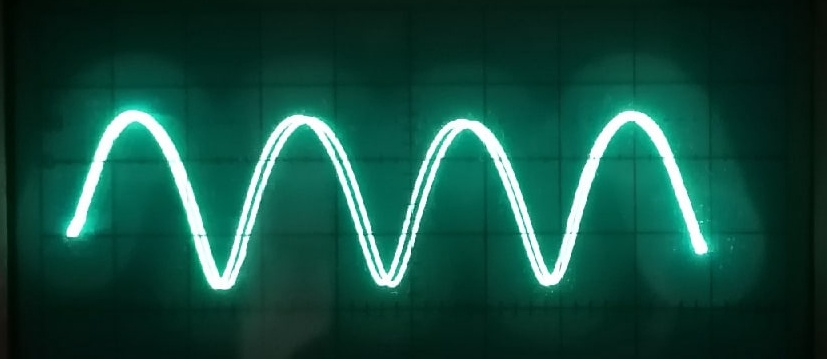
\includegraphics[width = 0.8\textwidth]{осциллограф.jpg}
\centering
\caption{Фигуры Лиссажу}
\end{figure}

Определим по фигурам Лиссажу полуволновое напряжение $U_{\lambda/2}$ как $\Delta U$, соответствующее переходу от максимума к минимуму сигнала на осциллограмме:\\
$U = U_{\lambda/2} = (0,42\pm 0,02)$ кВ, $U = U_{\lambda} = (0,87\pm 0,02)$кВ,$U = U_{\lambda/2} = (1,35\pm 0,02)$ кВ.
Отметим, что данные, полученные разными способами, сходятся в пределах $\sigma$

\subsection*{3.5 Переход к параллельной поляризации}

Пронаблюдаем, как изменится картина при параллельной поляризации, т.е. главная ось поляроида ориентирована вертикально: картина зеркально отобразится относительно оси Х

\section*{4. Выводы}

В работе изучена интерференция рассеянного света, прошедшего кристалл ниобата лития: получена зависимость квадрата радиуса темного кольца интерференционной картины от номера минимума $r_m^2(m)$. Двулучепреломление кристалла $n_o - n_e$ составляет $(98,2 \pm 0,1)\cdot10^{-3}$, это значение соответствует литиевым кристаллам. 
Рассмотрен эффект Поккельса: несколькими способами определено полуволновое напряжение, оно совпадает в пределах погрешности и равно $U_{\lambda/2} \approx 440$ В. Получены фигуры Лиссажу, отражающие зависимость интенсивности выходного сигнала от подаваемой амплитуды напряжения $I(U)$ при скрещенных и параллельных поляризациях.
	
	
\end{document}
